\chapter{Results and discussion}\label{cha:results}
In this chapter the results of the experiments detailed in the previous chapter are shown and discussed. The first section deals with pruning-related results. The next section is about categorical attributes and the final section pertains to the binary tree issue.

\section{Pruning}
In \autoref{cha:software_new}, pruning extensions were added to scikit-learn's decision tree implementations. More specifically, Reduced Error Pruning (REP) and Error Based Pruning (EBP) were implemented. In this section we evaluate how these pruning extensions affect the size of the tree (i.e., the number of nodes), the performance in terms of accuracy and the fitting and prediction speed.

%TODO next, Weka
\subsection{Tree size}
The mean size of the trees is shown as a heatmap in \autoref{fig:heat_nodes} for each dataset and each scikit-learn configuration. The values have been normalized by the mean size per dataset of unpruned trees. As such, the \emph{none} row which indicates that no pruning was performed is filled with 100\% values.

\begin{figure}[htp]
    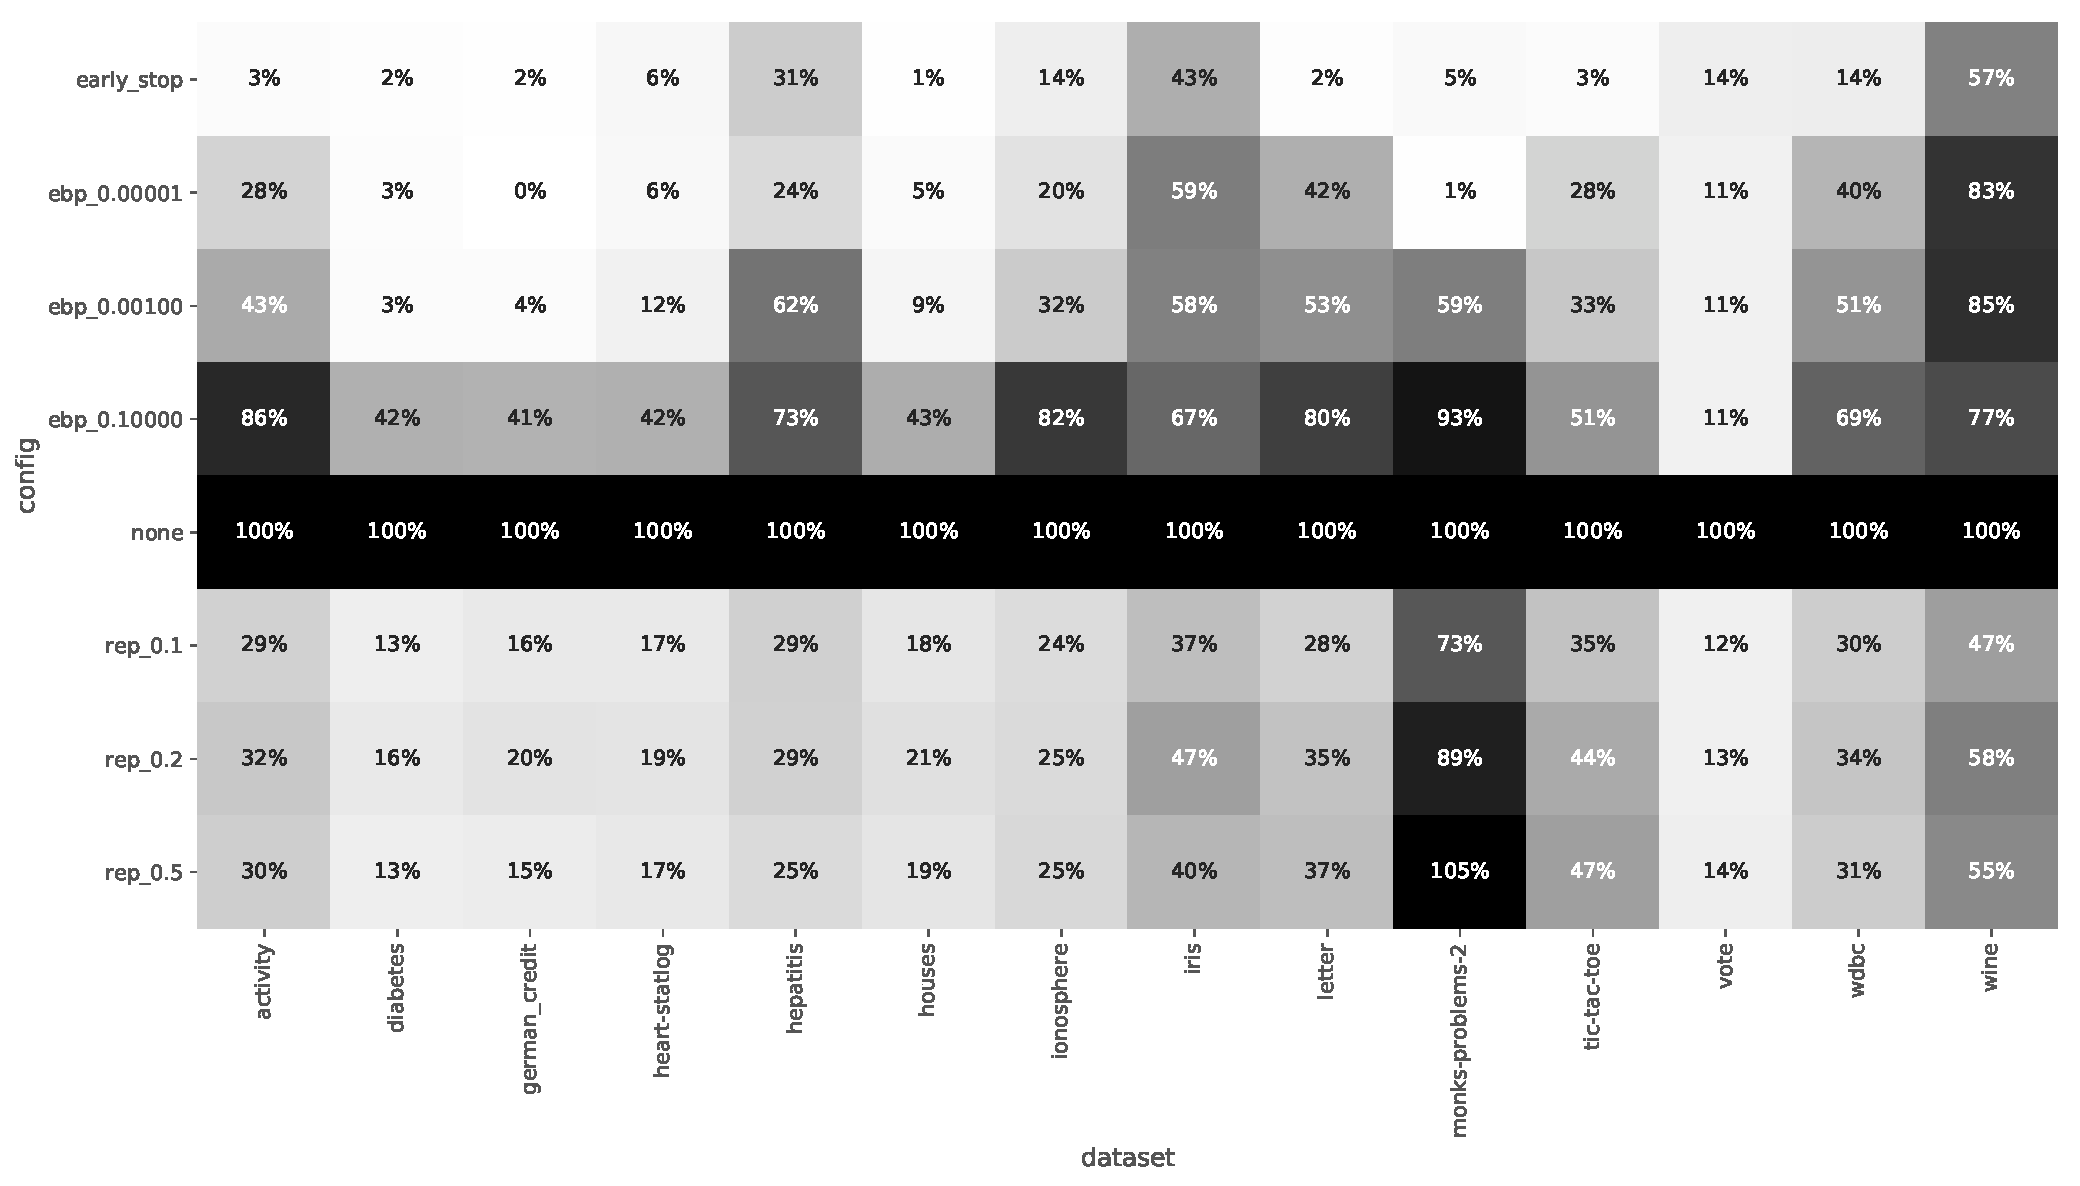
\includegraphics[width=\textwidth]{img/heatmap_n_nodes.pdf}
    \caption{Mean tree size per scikit-learn configuration and per dataset. The values have been normalized by the mean size per dataset of unpruned trees. Weka results are not included in this heatmap. The colour scale goes from 0\% (white) to 100\% (black).}%
    \label{fig:heat_nodes}
\end{figure}

One value exceeds 100\%. This is possible because the pruned trees are not derivatives of the unpruned trees. They are simply two different configurations that are tested independently of each other. In this specific case, Reduced Error Pruning was used with a validation set size equal to 50\% of the training set size. Since 10\% of the dataset was already set apart in the cross-validation procedure, only 45\% of the original data was left to train the tree. Compared to the other algorithms where larger fractions of training set remain, this can profoundly change the tree structure --- including its size --- before pruning. This size is unknown, but it must have been larger than the tree size of an unpruned tree trained on 90\% of the original data. Even after pruning, the former tree turned out to be larger than the latter.

The next observation is that the other rows in the heatmap are quite light, meaning that in general the tree sizes have been reduced greatly by the various pruning strategies. For Error Based Pruning, the confidence factor plays a large role in the amount of pruning that is performed. A very low confidence factor of $10^{-5}$ results in very aggressive pruning while a factor of $10^{-1}$ results in far less pruning. The validation set size of Reduced Error Pruning on the other hand does not have a clear impact on pruning aggression. A larger validation set only results in more reliable error estimates, but on average these estimates do not move in any particular direction.

Specifically for scikit-learn, a pseudo-pruning configuration is added that uses an early stopping criterion based on the \texttt{min\_samples\_leaf} parameter instead. This is what scikit-learn users do when pruning algorithms are unavailable. As discussed earlier, it is not easy to find a good value for this hyperparameter that performs similarly across a variety of datasets. In this case the result is very aggressive pruning except for datasets wine, iris and hepatitis. This is simply because the unpruned trees of these datasets were small to begin with, and this criterion aims for a low absolute number of nodes. The other configurations also score worse on these datasets because there is less potential for pruning if there are fewer nodes to start with. \autoref{fig:unpruned_sizes} gives an overview of the mean unpruned tree size of each dataset for both scikit-learn and Weka.

\begin{figure}[htp]
    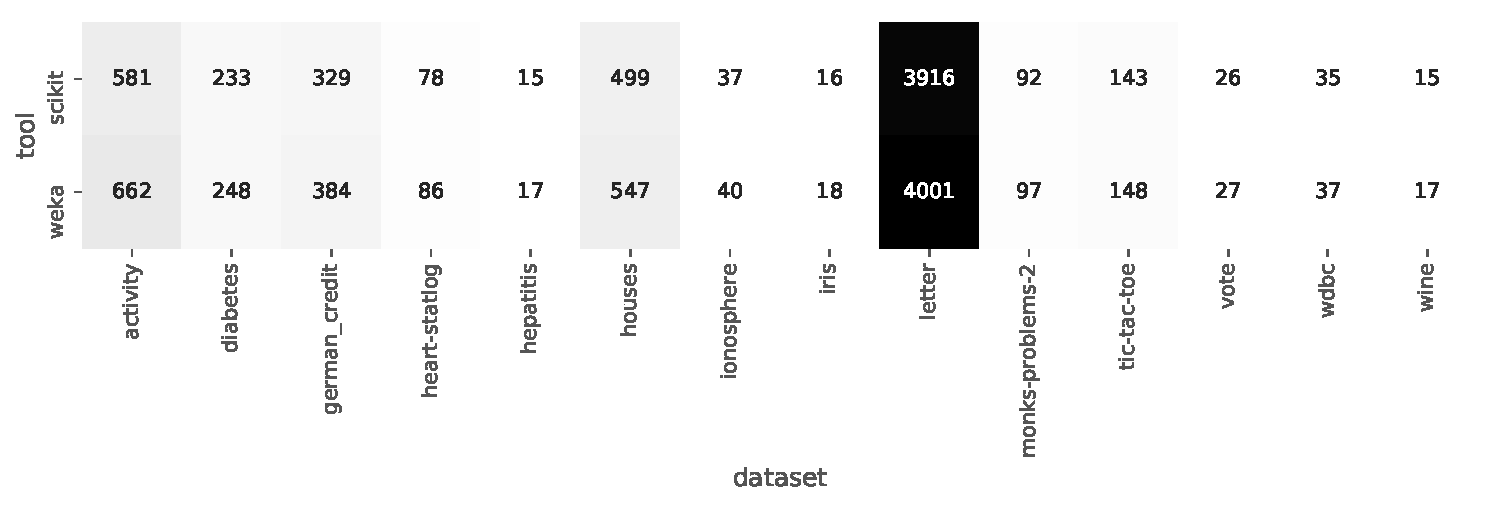
\includegraphics[width=\textwidth]{img/heatmap_n_nodes_unpruned.pdf}
    \caption{Mean size of unpruned trees (i.e., configuration \emph{none}) per dataset and per tool.}%
    \label{fig:unpruned_sizes}
\end{figure}

The first heatmap only showed results obtained from the scikit-learn configurations. The next step is to compare these results with those of Weka. \autoref{fig:heat_nodes_diff} visualizes the differences in number of nodes.

\begin{figure}[htp]
    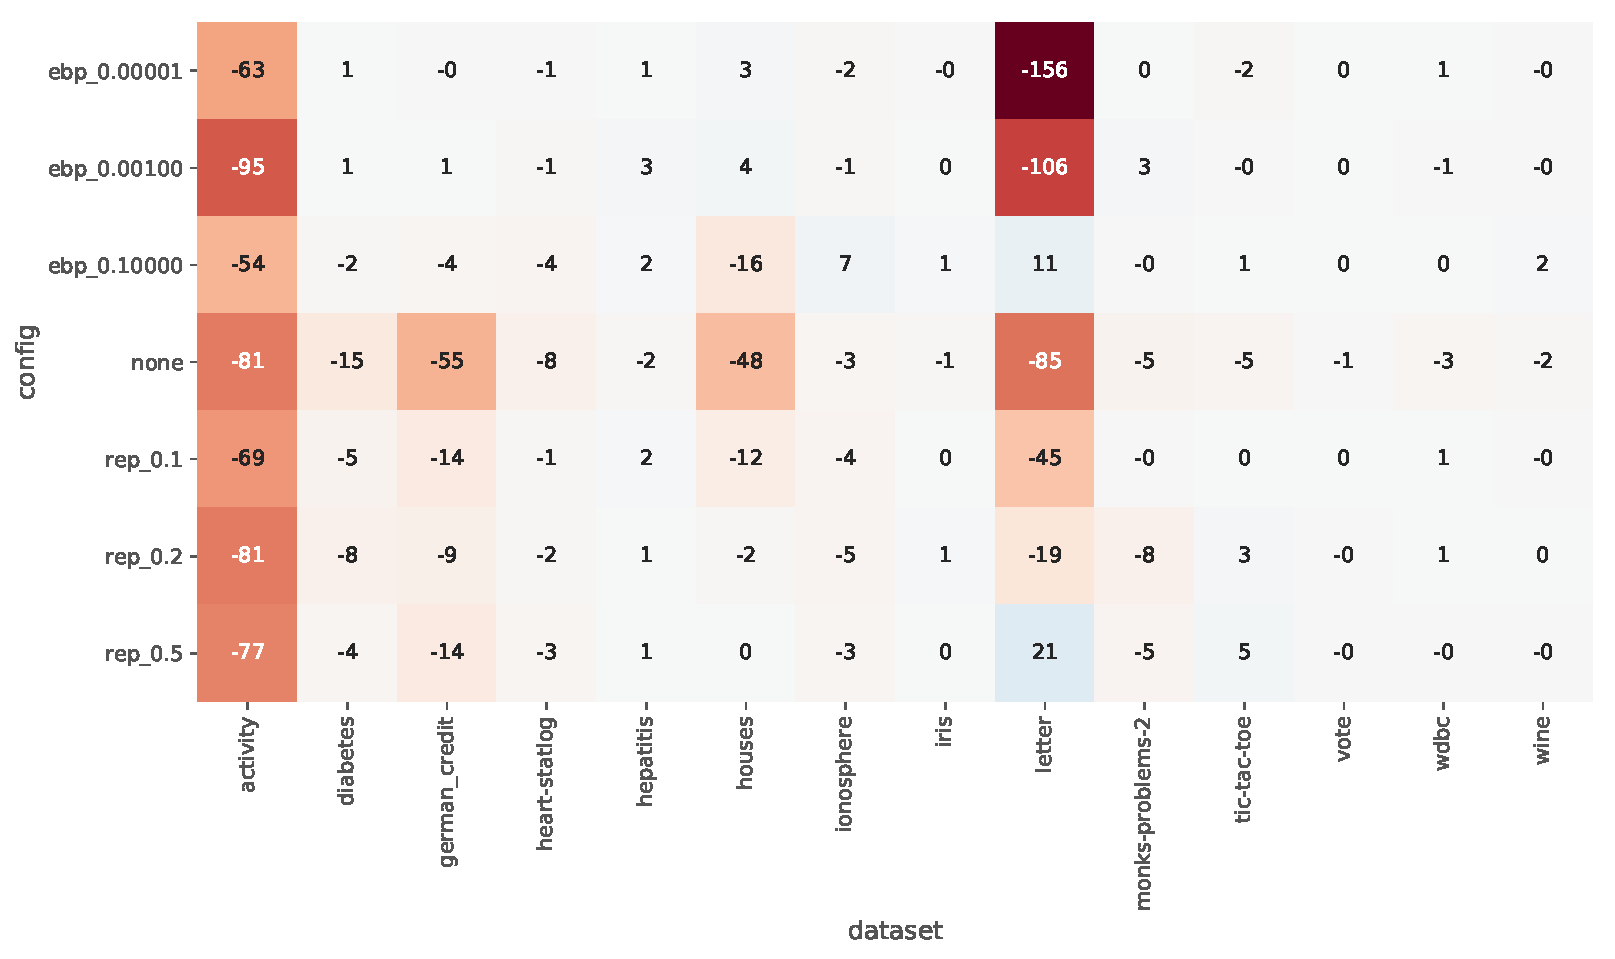
\includegraphics[width=\textwidth]{img/heatmap_n_nodes_diff.pdf}
    \caption{Differences between scikit-learn and Weka mean tree size per configuration and per dataset. Positive numbers indicate that scikit-learn generated larger trees on average compared to Weka, and vice versa.}%
    \label{fig:heat_nodes_diff}
\end{figure}

Most of the differences are minimal. The only configuration with some larger differences is the one where pruning is not applied. The previous heatmap showed us that mean unpruned tree size can be a multiple of any mean pruned tree size. Consequently, the differences in size between unpruned trees are also larger in absolute numbers. Also note that this configuration does not involve any relevant custom code developed for this thesis. Additionally, it is proof that CART and C4.5 (and their respective implementations) do not produce the exact same trees, even when configured very similarly.

Column-wise, the letter, activity datasets --- and to a lesser extent also houses and german\_credit datasets --- stand out. These are the datasets which on average generate the largest unpruned trees, as seen in \autoref{fig:unpruned_sizes}. Percentage-wise the effect pruning has on these four datasets is in line with the other datasets. As a result, their pruned trees are on average also large. This explains the larger absolute differences. When expressed relatively in percentages, the heatmap does not show any remarkable discrepancy between these four datasets and the rest.

In conclusion, the new pruning algorithms for scikit-learn decision trees behave as expected on the structure of the trees. The resulting sizes are grosso modo the same as when the experiments are performed in Weka. The next question is whether the performance also stays the same.

\subsection{Accuracy}
\autoref{fig:heat_acc} shows a heatmap of the mean accuracy per scikit-learn configuration and per dataset. The most important observation here is that all configurations except for early stopping behave very similarly, despite large differences in the amount of pruning. Of course this is the purpose of pruning: reduce model complexity without affecting performance too much. This goal is clearly accomplished. At the same time, a strong contrast with the performance of the early stopping criterion is revealed. Across the board, it performs worse than all real pruning configurations. In the previous section we learned that early stopping acts on the tree structure the same way an aggressive pruning algorithm would. The main difference is that in general the pruning strategies are in a better position to decide whether a node is really useful. In the end, a tree of the same size but with a better node selection performs better than a tree that stopped growing prematurely because of some very generic criteria.

\begin{figure}[htp]
    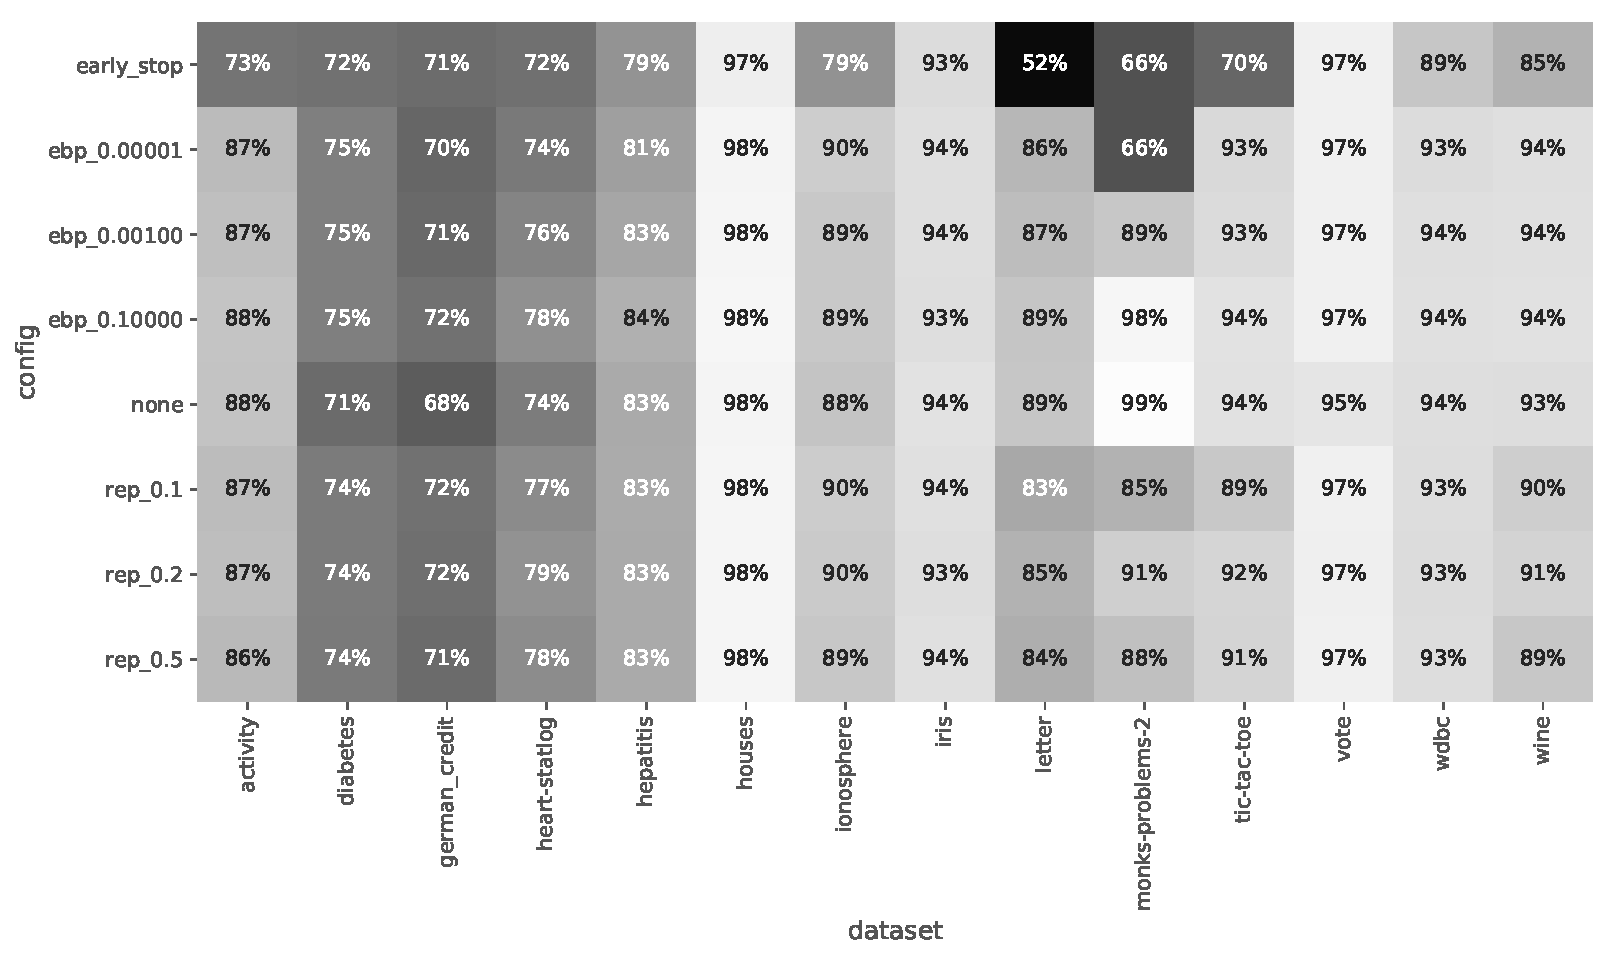
\includegraphics[width=\textwidth]{img/heatmap_accuracy.pdf}
    \caption{Mean accuracy per scikit-learn configuration and per dataset. Weka results are not included in this heatmap. The colour scale goes from 50\% (black) to 100\% (white).}%
    \label{fig:heat_acc}
\end{figure}

This heatmap also clearly shows that accuracy is strongly dependent on the dataset. Not all datasets can be modelled equally well with trees (or with any classifier for that matter). Differences in class balance also exist between datasets. Accuracy as a metric can be biased when the classes are strongly unbalanced. Alternative metrics such as the F1-score are better suited in such scenarios. A similar heatmap as shown here was generated using this F1-score, but it is not included because the results were almost identical.

A small note about the result of the \emph{ebp\_0.00001} configuration on the monks dataset: the low value for the confidence value hyperparameter makes the pruner very aggressive. In this case so much that the pruned tree consists of only one node that predicts the majority class all the time.

\begin{figure}[htp]
    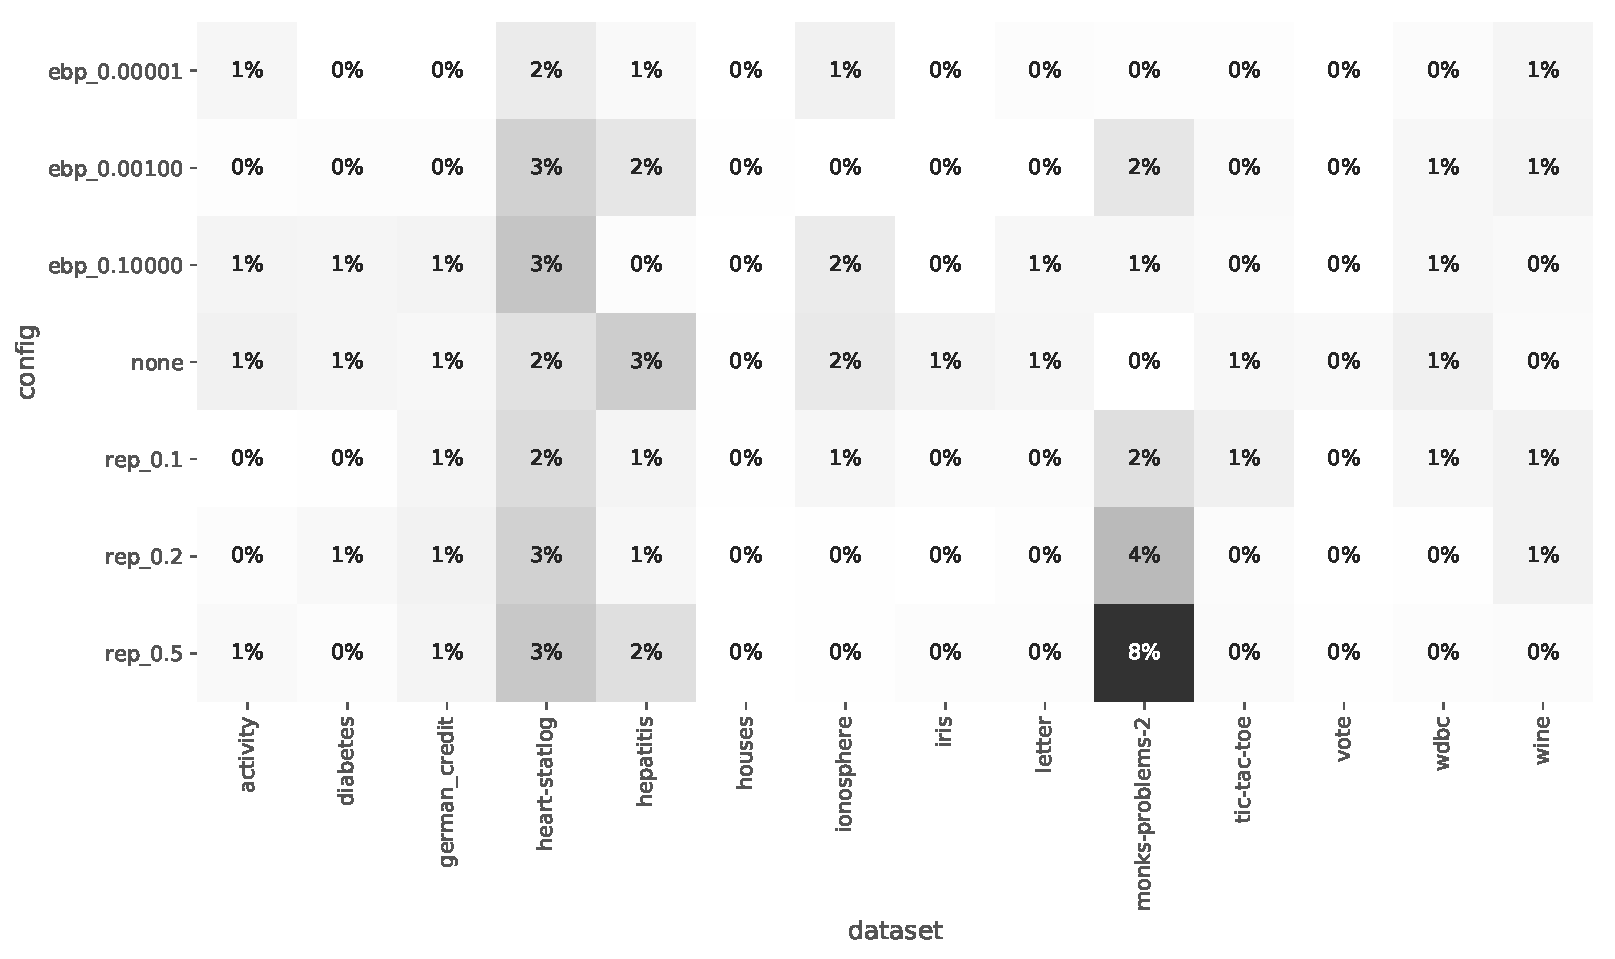
\includegraphics[width=\textwidth]{img/heatmap_accuracy_diff.pdf}
    \caption{Differences in percentage points (pp) between scikit-learn and Weka mean accuracy scores per configuration and per dataset. Positive numbers indicate that scikit-learn had a higher accuracy on average compared to Weka, and vice versa.}%
    \label{fig:heat_acc_diff}
\end{figure}

\autoref{fig:heat_acc_diff} reveals that these scikit-learn accuracy scores are almost perfectly in line with the Weka scores. The only real concern is the eight percentage points difference in favour of scikit-learn on the monks dataset using Reduced Error Pruning with a 50\% validation set size. Depending on which half of the data was withheld from training, the tree structure can vary dramatically. Consequently, the accuracy can vary a lot as well.
%TODO std similar, dig deeper

The same figure also reveals that the accuracy scores on the activity dataset are almost identical between scikit-learn and Weka configurations. Even the unpruned configurations perform almost identical. This contradicts earlier reports that noticed a significant difference in performance between the two tools. We cannot reproduce this issue.

\subsection{Fitting and training time}
One last performance aspect of performance that we need to evaluate is the time taken (in milliseconds) to fit the tree and predict results with it. \autoref{fig:heat_fit} and \autoref{fig:heat_fit_diff} show the fitting time results in scikit-learn and the difference in fitting time between Weka and scikit-learn respectively. In both plots the datasets that require large trees once again stand out. This makes sense: building larger trees takes more time than building smaller trees. Weka performs worse in this aspect on such datasets. On other datasets the difference is negligible. Comparing the performance of a Java program to a Python program in terms of speed is like comparing apples and oranges, so we will not dive deeper into this topic.

\begin{figure}[htp]
    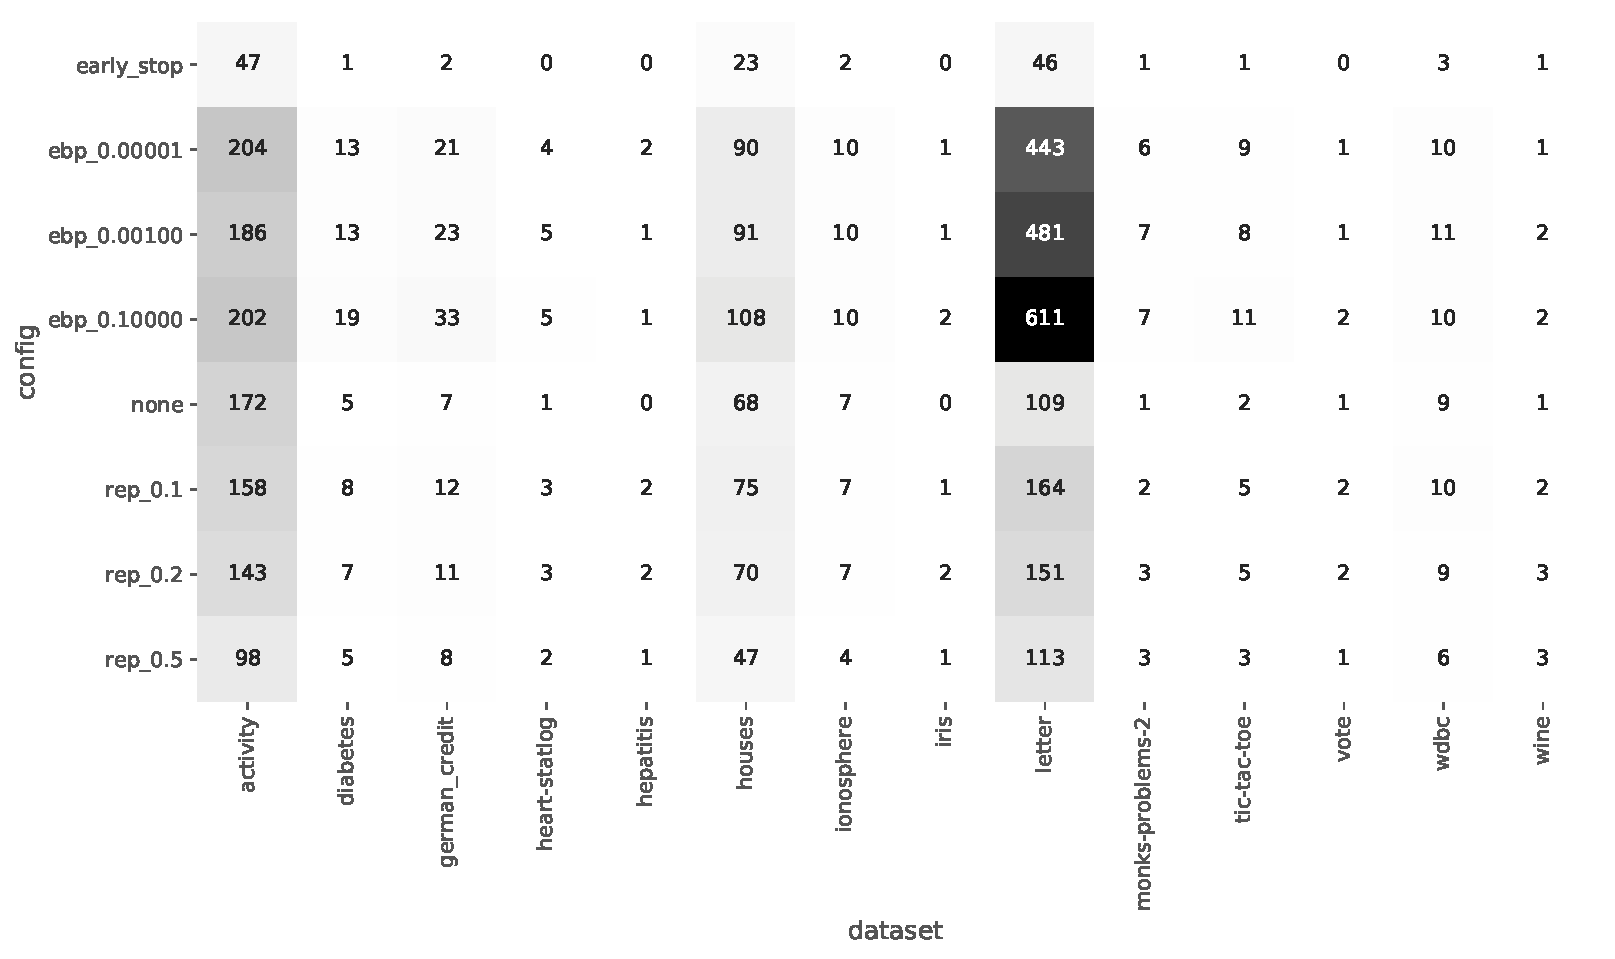
\includegraphics[width=\textwidth]{img/heatmap_fit_time.pdf}
    \caption{Mean fitting times in milliseconds per scikit-learn configuration and per dataset. Weka results are not included in this heatmap.}%
    \label{fig:heat_fit}
\end{figure}

\begin{figure}[htp]
    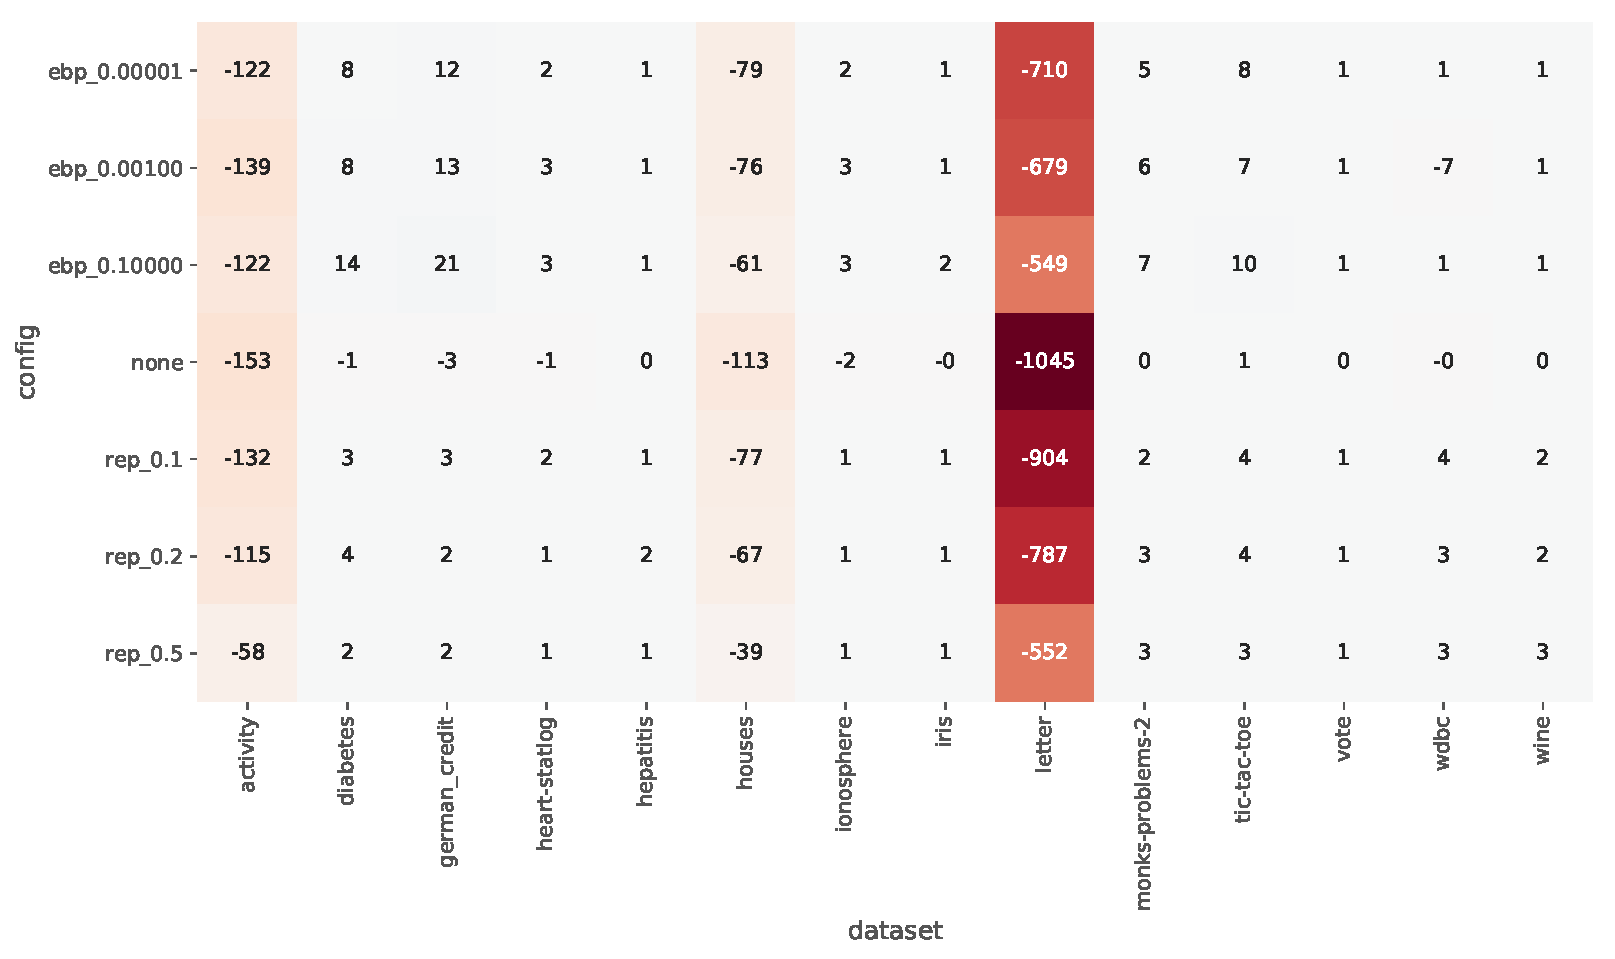
\includegraphics[width=\textwidth]{img/heatmap_fit_time_diff.pdf}
    \caption{Differences in mean fitting times in milliseconds between scikit-learn and Weka per configuration and per dataset. Positive numbers indicate that scikit-learn took longer on average compared to Weka, and vice versa.}%
    \label{fig:heat_fit_diff}
\end{figure}

The early stopping configuration performs the fastest fits, which is not surprising at all, but it comes at a cost in accuracy as we learned before. Pruning configurations should fit slower than the unpruned configuration because an extra step is added in this procedure. However, the results show that this is not always the case, especially when Reduced Error Pruning is applied. One possible explanation is that fewer observations are used during the growth phase. If the extra pruning phase is performed fast enough, the net result could still be faster compared to when no pruning was applied. The results support this hypothesis: the larger the validation set size, the lower the total fitting time. The Error Based Pruning configurations on the other hand behave as expected since they do not set data aside in a validation set. In that case, adding the pruning step increases total fit time. Note that these tendencies are only clearly visible when the total fitting time is large enough. In other cases, the results are lost in statistical noise.

Heatmaps of (differences in) mean prediction times are not included in this text because they do not add much value. The results are all in the range of 0--2ms, except for the letter database which takes 2--3ms for scikit-learn and 7--8ms for Weka. Due to the very low values, comparison across configurations is almost impossible and at the same time irrelevant.

\subsection{Summary}
This concludes the performance analysis of the new pruning algorithms. As expected, tree size plays a major role in explaining the subtle differences in the results. The heatmaps that show the difference in various performance aspects all reveal that scikit-learn performs very similarly to --- and sometimes even better than --- Weka. This means we successfully increased the feature parity between the two tools, which was one of the main goals of this thesis.

\section{Categorical attributes}

\section{Binary versus non-binary trees}
% Weka: binary vs non binary - significant differences
%   binary -> non-binary
%   tic-tac-toe: 
%       41.36 -> 10 nodes
%       21.18 -> 7 leaves
%       92.79 -> 68.96 accuracy
%       0.93 -> 0.71 F1
%   monks: always tree with only root node, no F1 score
%   activity: 85.66 -> 84.43 accuracy (no significant difference in F1)
% ==> non-binary same or disadvantage

\section{Conclusion}
